\documentclass[twoside]{book}

% Packages required by doxygen
\usepackage{calc}
\usepackage{doxygen}
\usepackage{graphicx}
\usepackage[utf8]{inputenc}
\usepackage{makeidx}
\usepackage{multicol}
\usepackage{multirow}
\usepackage{textcomp}
\usepackage[table]{xcolor}

% Font selection
\usepackage[T1]{fontenc}
\usepackage{mathptmx}
\usepackage[scaled=.90]{helvet}
\usepackage{courier}
\usepackage{amssymb}
\usepackage{sectsty}
\renewcommand{\familydefault}{\sfdefault}
\allsectionsfont{%
  \fontseries{bc}\selectfont%
  \color{darkgray}%
}
\renewcommand{\DoxyLabelFont}{%
  \fontseries{bc}\selectfont%
  \color{darkgray}%
}

% Page & text layout
\usepackage{geometry}
\geometry{%
  a4paper,%
  top=2.5cm,%
  bottom=2.5cm,%
  left=2.5cm,%
  right=2.5cm%
}
\tolerance=750
\hfuzz=15pt
\hbadness=750
\setlength{\emergencystretch}{15pt}
\setlength{\parindent}{0cm}
\setlength{\parskip}{0.2cm}
\makeatletter
\renewcommand{\paragraph}{%
  \@startsection{paragraph}{4}{0ex}{-1.0ex}{1.0ex}{%
    \normalfont\normalsize\bfseries\SS@parafont%
  }%
}
\renewcommand{\subparagraph}{%
  \@startsection{subparagraph}{5}{0ex}{-1.0ex}{1.0ex}{%
    \normalfont\normalsize\bfseries\SS@subparafont%
  }%
}
\makeatother

% Headers & footers
\usepackage{fancyhdr}
\pagestyle{fancyplain}
\fancyhead[LE]{\fancyplain{}{\bfseries\thepage}}
\fancyhead[CE]{\fancyplain{}{}}
\fancyhead[RE]{\fancyplain{}{\bfseries\leftmark}}
\fancyhead[LO]{\fancyplain{}{\bfseries\rightmark}}
\fancyhead[CO]{\fancyplain{}{}}
\fancyhead[RO]{\fancyplain{}{\bfseries\thepage}}
\fancyfoot[LE]{\fancyplain{}{}}
\fancyfoot[CE]{\fancyplain{}{}}
\fancyfoot[RE]{\fancyplain{}{\bfseries\scriptsize Generated on Tue Mar 22 2016 10\-:02\-:07 for Q\-Sticky\-Button by Doxygen }}
\fancyfoot[LO]{\fancyplain{}{\bfseries\scriptsize Generated on Tue Mar 22 2016 10\-:02\-:07 for Q\-Sticky\-Button by Doxygen }}
\fancyfoot[CO]{\fancyplain{}{}}
\fancyfoot[RO]{\fancyplain{}{}}
\renewcommand{\footrulewidth}{0.4pt}
\renewcommand{\chaptermark}[1]{%
  \markboth{#1}{}%
}
\renewcommand{\sectionmark}[1]{%
  \markright{\thesection\ #1}%
}

% Indices & bibliography
\usepackage{natbib}
\usepackage[titles]{tocloft}
\setcounter{tocdepth}{3}
\setcounter{secnumdepth}{5}
\makeindex

% Hyperlinks (required, but should be loaded last)
\usepackage{ifpdf}
\ifpdf
  \usepackage[pdftex,pagebackref=true]{hyperref}
\else
  \usepackage[ps2pdf,pagebackref=true]{hyperref}
\fi
\hypersetup{%
  colorlinks=true,%
  linkcolor=blue,%
  citecolor=blue,%
  unicode%
}

% Custom commands
\newcommand{\clearemptydoublepage}{%
  \newpage{\pagestyle{empty}\cleardoublepage}%
}


%===== C O N T E N T S =====

\begin{document}

% Titlepage & ToC
\hypersetup{pageanchor=false}
\pagenumbering{roman}
\begin{titlepage}
\vspace*{7cm}
\begin{center}%
{\Large Q\-Sticky\-Button \\[1ex]\large 0.\-1.\-0 }\\
\vspace*{1cm}
{\large Generated by Doxygen 1.8.6}\\
\vspace*{0.5cm}
{\small Tue Mar 22 2016 10:02:07}\\
\end{center}
\end{titlepage}
\clearemptydoublepage
\tableofcontents
\clearemptydoublepage
\pagenumbering{arabic}
\hypersetup{pageanchor=true}

%--- Begin generated contents ---
\chapter{Main Page}
\label{index}\hypertarget{index}{}This is the documentation of a custom widget for the \href{http://www.qt.io/}{\tt Qt Framework}. It contains the actual documentation of the Q\-Sticky\-Widget and an example implementation with all the capabilities of the \hyperlink{class_q_sticky_button}{Q\-Sticky\-Button} used.\hypertarget{index_button_example_section}{}\section{The button}\label{index_button_example_section}
\begin{DoxyParagraph}{The button}
Below is the \hyperlink{class_q_sticky_button}{Q\-Sticky\-Button} shown as an animated image. This shows both the unlocked and locked state of the button. 
\end{DoxyParagraph}
\begin{DoxyParagraph}{Implemented button.}
Below is the example implementation shown, using all the capabilities of the \hyperlink{class_q_sticky_button}{Q\-Sticky\-Button}. 
\end{DoxyParagraph}
\hypertarget{index_usage_section}{}\section{Usage}\label{index_usage_section}

\begin{DoxyEnumerate}
\item Adding the source files to the destination Qt Project.
\begin{DoxyItemize}
\item The needed source files should be placed in the source code directory of a project. See the file tree below, which is from the example implementation. Project folder\-:
\begin{DoxyItemize}
\item Q\-Sticky\-Button.\-pro
\item Q\-Sticky\-Button.\-qrc
\item img
\begin{DoxyItemize}
\item Lock\-Closed.\-png
\item Lock\-Opened.\-png
\end{DoxyItemize}
\item source
\begin{DoxyItemize}
\item \hyperlink{_main_window_8h}{Main\-Window.\-h}
\item \hyperlink{_q_sticky_button_8h}{Q\-Sticky\-Button.\-h}
\item src
\begin{DoxyItemize}
\item \hyperlink{_main_window_8cpp}{Main\-Window.\-cpp}
\item \hyperlink{_q_sticky_button_8cpp}{Q\-Sticky\-Button.\-cpp}
\item main.\-cpp
\end{DoxyItemize}
\end{DoxyItemize}
\item ui
\begin{DoxyItemize}
\item Main\-Window.\-ui
\item Q\-Sticky\-Button.\-ui
\end{DoxyItemize}
\end{DoxyItemize}

Note that the image files ({\ttfamily img/\-Lock\-Closed.\-png}, and {\ttfamily img/\-Lock\-Opened.\-png}) also need to be placed in the source code directory. When the image files are in a different directory than {\ttfamily img}, the images may need to be re-\/linked to the resource file.
\item Add {\ttfamily Q\-Sticky\-Button.\-ui}, \hyperlink{_q_sticky_button_8h}{Q\-Sticky\-Button.\-h}, \hyperlink{_q_sticky_button_8cpp}{Q\-Sticky\-Button.\-cpp}, and {\ttfamily Q\-Sticky\-Button.\-qrc} to the Qt project as shown below. 
\end{DoxyItemize}
\item Create a standard widget in the destination {\ttfamily ui}.
\item Promote the standard widget to the \hyperlink{class_q_sticky_button}{Q\-Sticky\-Button}.
\begin{DoxyItemize}
\item Right click on the {\ttfamily Q\-Widget} and go to {\ttfamily Promote to ...}
\item As {\ttfamily Promoted class name} enter\begin{DoxyVerb}QStickyButton \end{DoxyVerb}

\item It will automatically select {\ttfamily \hyperlink{_q_sticky_button_8h}{Q\-Sticky\-Button.\-h}} as {\ttfamily Header file}
\item Click on {\ttfamily Promote}
\end{DoxyItemize}
\item Add the title property to the \hyperlink{class_q_sticky_button}{Q\-Sticky\-Button}.
\begin{DoxyItemize}
\item Select {\ttfamily Add Dynamic Property} in the {\ttfamily Property Editor} (just below the {\ttfamily Object Inspector}) and add a {\ttfamily String...}
\item Enter\begin{DoxyVerb}title \end{DoxyVerb}
 as {\ttfamily Property Name} and make sure that the {\ttfamily Property Type} is set to {\ttfamily String}.
\item Click {\ttfamily O\-K} to add the dynamic property to the \hyperlink{class_q_sticky_button}{Q\-Sticky\-Button}.
\item In the {\ttfamily Property Editor} scroll all the way to the bottom to see the created property, and set a title
\end{DoxyItemize}
\item Connect and use the button. Now the button can be connected to a {\ttfamily slot}, for example
\begin{DoxyCode}
\textcolor{keywordtype}{void} userFunction(\textcolor{keywordtype}{bool} stickyButtonState); 
\end{DoxyCode}
 by adding
\begin{DoxyCode}
connect(ui->stickyButton, &\hyperlink{class_q_sticky_button_ab47e7e8f739b82d34cceb4f5f2ccb101}{QStickyButton::toggled},
        \textcolor{keyword}{this}, &\hyperlink{class_main_window_a648ea2bfab3eef2287c28a76a8e86948}{MainWindow::userFunction}); 
\end{DoxyCode}
 to the window constructor.
\end{DoxyEnumerate}\hypertarget{index_licensing}{}\section{Licensing}\label{index_licensing}
G\-N\-U General Public License version 3 or later, as published by the Free Software Foundation. Modification and redistribution are permitted according to the terms of the G\-P\-L. The short license can be found in the \hyperlink{license}{license} section, and the full license can be found in the {\ttfamily L\-I\-C\-E\-N\-S\-E} file. 
\chapter{License}
\label{license}
\hypertarget{license}{}
Licence information.

Copyright (c) 2016 Jeroen de Bruijn \href{mailto:vidavidorra4pub@gmail.com}{\tt vidavidorra4pub@gmail.\-com}

This program is free software\-: you can redistribute it and/or modify it under the terms of the G\-N\-U General Public License as published by the Free Software Foundation, either version 3 of the License, or (at your option) any later version.

This program is distributed in the hope that it will be useful, but W\-I\-T\-H\-O\-U\-T A\-N\-Y W\-A\-R\-R\-A\-N\-T\-Y; without even the implied warranty of M\-E\-R\-C\-H\-A\-N\-T\-A\-B\-I\-L\-I\-T\-Y or F\-I\-T\-N\-E\-S\-S F\-O\-R A P\-A\-R\-T\-I\-C\-U\-L\-A\-R P\-U\-R\-P\-O\-S\-E. See the G\-N\-U General Public License for more details.

You should have received a copy of the G\-N\-U General Public License along with this program. If not, see \href{http://www.gnu.org/licenses/}{\tt http\-://www.\-gnu.\-org/licenses/}. 
\chapter{Hierarchical Index}
\section{Class Hierarchy}
This inheritance list is sorted roughly, but not completely, alphabetically\-:\begin{DoxyCompactList}
\item Q\-Main\-Window\begin{DoxyCompactList}
\item \contentsline{section}{Main\-Window}{\pageref{class_main_window}}{}
\end{DoxyCompactList}
\item Q\-Widget\begin{DoxyCompactList}
\item \contentsline{section}{Q\-Sticky\-Button}{\pageref{class_q_sticky_button}}{}
\end{DoxyCompactList}
\end{DoxyCompactList}

\chapter{Class Index}
\section{Class List}
Here are the classes, structs, unions and interfaces with brief descriptions\-:\begin{DoxyCompactList}
\item\contentsline{section}{\hyperlink{class_main_window}{Main\-Window} \\*Shows an example implementation of the Q\-S\-Ticky\-Button with all the capabilities used }{\pageref{class_main_window}}{}
\item\contentsline{section}{\hyperlink{class_q_sticky_button}{Q\-Sticky\-Button} \\*Implements a custom button with click and hold capability }{\pageref{class_q_sticky_button}}{}
\end{DoxyCompactList}

\chapter{File Index}
\section{File List}
Here is a list of all documented files with brief descriptions\-:\begin{DoxyCompactList}
\item\contentsline{section}{source/\hyperlink{_main_window_8h}{Main\-Window.\-h} \\*Example implementation of the \hyperlink{class_q_sticky_button}{Q\-Sticky\-Button} }{\pageref{_main_window_8h}}{}
\item\contentsline{section}{source/\hyperlink{_q_sticky_button_8h}{Q\-Sticky\-Button.\-h} \\*Sticky button that has click and hold capability }{\pageref{_q_sticky_button_8h}}{}
\item\contentsline{section}{source/src/\hyperlink{_main_window_8cpp}{Main\-Window.\-cpp} \\*Example implementation of the \hyperlink{class_q_sticky_button}{Q\-Sticky\-Button} }{\pageref{_main_window_8cpp}}{}
\item\contentsline{section}{source/src/\hyperlink{_q_sticky_button_8cpp}{Q\-Sticky\-Button.\-cpp} \\*Sticky button that has click and hold capability }{\pageref{_q_sticky_button_8cpp}}{}
\end{DoxyCompactList}

\chapter{Class Documentation}
\hypertarget{class_main_window}{\section{Main\-Window Class Reference}
\label{class_main_window}\index{Main\-Window@{Main\-Window}}
}


The \hyperlink{class_main_window}{Main\-Window} class shows an example implementation of the Q\-S\-Ticky\-Button with all the capabilities used.  




{\ttfamily \#include $<$Main\-Window.\-h$>$}



Inheritance diagram for Main\-Window\-:
\nopagebreak
\begin{figure}[H]
\begin{center}
\leavevmode
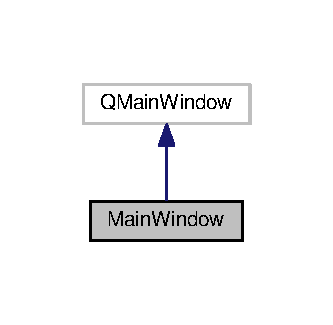
\includegraphics[width=160pt]{class_main_window__inherit__graph}
\end{center}
\end{figure}


Collaboration diagram for Main\-Window\-:
\nopagebreak
\begin{figure}[H]
\begin{center}
\leavevmode
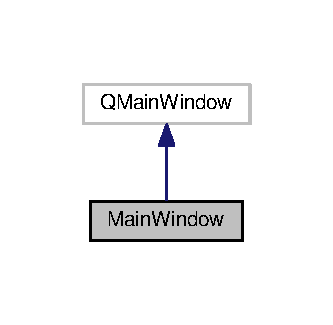
\includegraphics[width=160pt]{class_main_window__coll__graph}
\end{center}
\end{figure}
\subsection*{Public Slots}
\begin{DoxyCompactItemize}
\item 
void \hyperlink{class_main_window_a648ea2bfab3eef2287c28a76a8e86948}{user\-Function} (bool sticky\-Button\-State)
\begin{DoxyCompactList}\small\item\em Example user function that is called when the state of the \hyperlink{class_q_sticky_button}{Q\-Sticky\-Button} has changed. \end{DoxyCompactList}\end{DoxyCompactItemize}
\subsection*{Public Member Functions}
\begin{DoxyCompactItemize}
\item 
\hyperlink{class_main_window_a8b244be8b7b7db1b08de2a2acb9409db}{Main\-Window} (Q\-Widget $\ast$parent=0)
\begin{DoxyCompactList}\small\item\em Default constructor. \end{DoxyCompactList}\item 
\hyperlink{class_main_window_ae98d00a93bc118200eeef9f9bba1dba7}{$\sim$\-Main\-Window} ()
\begin{DoxyCompactList}\small\item\em Default destructor. \end{DoxyCompactList}\end{DoxyCompactItemize}


\subsection{Detailed Description}
The \hyperlink{class_main_window}{Main\-Window} class shows an example implementation of the Q\-S\-Ticky\-Button with all the capabilities used. 

Definition at line 48 of file Main\-Window.\-h.



\subsection{Constructor \& Destructor Documentation}
\hypertarget{class_main_window_a8b244be8b7b7db1b08de2a2acb9409db}{\index{Main\-Window@{Main\-Window}!Main\-Window@{Main\-Window}}
\index{Main\-Window@{Main\-Window}!MainWindow@{Main\-Window}}
\subsubsection[{Main\-Window}]{\setlength{\rightskip}{0pt plus 5cm}Main\-Window\-::\-Main\-Window (
\begin{DoxyParamCaption}
\item[{Q\-Widget $\ast$}]{parent = {\ttfamily 0}}
\end{DoxyParamCaption}
)\hspace{0.3cm}{\ttfamily [explicit]}}}\label{class_main_window_a8b244be8b7b7db1b08de2a2acb9409db}


Default constructor. 

The system's default constructor. 

Definition at line 35 of file Main\-Window.\-cpp.


\begin{DoxyCode}
35                                       :
36     QMainWindow(parent),
37     ui(\textcolor{keyword}{new} Ui::MainWindow)
38 \{
39     ui->setupUi(\textcolor{keyword}{this});
40 
41     connect(ui->stickyButton, &\hyperlink{class_q_sticky_button_ab47e7e8f739b82d34cceb4f5f2ccb101}{QStickyButton::toggled},
42                 \textcolor{keyword}{this}, &\hyperlink{class_main_window_a648ea2bfab3eef2287c28a76a8e86948}{MainWindow::userFunction});
43 \}
\end{DoxyCode}
\hypertarget{class_main_window_ae98d00a93bc118200eeef9f9bba1dba7}{\index{Main\-Window@{Main\-Window}!$\sim$\-Main\-Window@{$\sim$\-Main\-Window}}
\index{$\sim$\-Main\-Window@{$\sim$\-Main\-Window}!MainWindow@{Main\-Window}}
\subsubsection[{$\sim$\-Main\-Window}]{\setlength{\rightskip}{0pt plus 5cm}Main\-Window\-::$\sim$\-Main\-Window (
\begin{DoxyParamCaption}
{}
\end{DoxyParamCaption}
)}}\label{class_main_window_ae98d00a93bc118200eeef9f9bba1dba7}


Default destructor. 

The system's default destructor. 

Definition at line 45 of file Main\-Window.\-cpp.


\begin{DoxyCode}
46 \{
47     \textcolor{keyword}{delete} ui;
48 \}
\end{DoxyCode}


\subsection{Member Function Documentation}
\hypertarget{class_main_window_a648ea2bfab3eef2287c28a76a8e86948}{\index{Main\-Window@{Main\-Window}!user\-Function@{user\-Function}}
\index{user\-Function@{user\-Function}!MainWindow@{Main\-Window}}
\subsubsection[{user\-Function}]{\setlength{\rightskip}{0pt plus 5cm}void Main\-Window\-::user\-Function (
\begin{DoxyParamCaption}
\item[{bool}]{sticky\-Button\-State}
\end{DoxyParamCaption}
)\hspace{0.3cm}{\ttfamily [slot]}}}\label{class_main_window_a648ea2bfab3eef2287c28a76a8e86948}


Example user function that is called when the state of the \hyperlink{class_q_sticky_button}{Q\-Sticky\-Button} has changed. 


\begin{DoxyParams}{Parameters}
{\em sticky\-Button\-State} & The current state of the \hyperlink{class_q_sticky_button}{Q\-Sticky\-Button}. \\
\hline
\end{DoxyParams}


Definition at line 50 of file Main\-Window.\-cpp.


\begin{DoxyCode}
51 \{
52     QString boolText = stickyButtonState ? \textcolor{stringliteral}{"true"} : \textcolor{stringliteral}{"false"};
53     ui->buttonStateLine->setText(boolText);
54 \}
\end{DoxyCode}


The documentation for this class was generated from the following files\-:\begin{DoxyCompactItemize}
\item 
source/\hyperlink{_main_window_8h}{Main\-Window.\-h}\item 
source/src/\hyperlink{_main_window_8cpp}{Main\-Window.\-cpp}\end{DoxyCompactItemize}

\hypertarget{class_q_sticky_button}{\section{Q\-Sticky\-Button Class Reference}
\label{class_q_sticky_button}\index{Q\-Sticky\-Button@{Q\-Sticky\-Button}}
}


The \hyperlink{class_q_sticky_button}{Q\-Sticky\-Button} class implements a custom button with click and hold capability.  




{\ttfamily \#include $<$Q\-Sticky\-Button.\-h$>$}



Inheritance diagram for Q\-Sticky\-Button\-:
\nopagebreak
\begin{figure}[H]
\begin{center}
\leavevmode
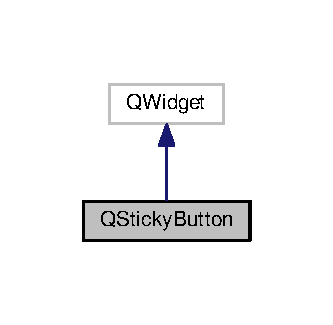
\includegraphics[width=160pt]{class_q_sticky_button__inherit__graph}
\end{center}
\end{figure}


Collaboration diagram for Q\-Sticky\-Button\-:
\nopagebreak
\begin{figure}[H]
\begin{center}
\leavevmode
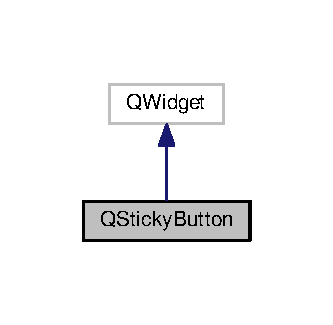
\includegraphics[width=160pt]{class_q_sticky_button__coll__graph}
\end{center}
\end{figure}
\subsection*{Public Slots}
\begin{DoxyCompactItemize}
\item 
void \hyperlink{class_q_sticky_button_a694a4a05275faf028d6e29e2a10fe059}{set\-Checked} (bool pressed)
\begin{DoxyCompactList}\small\item\em Set the checked state of the sticky button. \end{DoxyCompactList}\item 
bool \hyperlink{class_q_sticky_button_a33b2e4842a6c2ddd55e0c9f5425942ba}{is\-Checked} () const 
\begin{DoxyCompactList}\small\item\em Get the checked or pressed status of the sticky button. \end{DoxyCompactList}\end{DoxyCompactItemize}
\subsection*{Signals}
\begin{DoxyCompactItemize}
\item 
void \hyperlink{class_q_sticky_button_ab47e7e8f739b82d34cceb4f5f2ccb101}{toggled} (bool checked) const 
\begin{DoxyCompactList}\small\item\em Toggled signal for the lockbutton. \end{DoxyCompactList}\end{DoxyCompactItemize}
\subsection*{Public Member Functions}
\begin{DoxyCompactItemize}
\item 
\hyperlink{class_q_sticky_button_ac2c3029091cc02ebcb32897511adbcb1}{Q\-Sticky\-Button} (Q\-Widget $\ast$parent=0)
\begin{DoxyCompactList}\small\item\em Default constructor. \end{DoxyCompactList}\item 
\hyperlink{class_q_sticky_button_ad5912bd79a895579588961f9e9d73572}{$\sim$\-Q\-Sticky\-Button} ()
\begin{DoxyCompactList}\small\item\em Default destructor. \end{DoxyCompactList}\item 
void \hyperlink{class_q_sticky_button_a5bac733cac165aac0b181a5b5d5976a3}{set\-Title} (const Q\-String \&\hyperlink{class_q_sticky_button_ad4ce92181d1cceab37cecdce54249e24}{title})
\begin{DoxyCompactList}\small\item\em Set the title of the pushbutton. \end{DoxyCompactList}\item 
Q\-String \hyperlink{class_q_sticky_button_a32a1b2b10c91b85f96e8e01876a81c18}{title} () const 
\begin{DoxyCompactList}\small\item\em Get the title of the pushbutton. \end{DoxyCompactList}\end{DoxyCompactItemize}
\subsection*{Properties}
\begin{DoxyCompactItemize}
\item 
Q\-String \hyperlink{class_q_sticky_button_ad4ce92181d1cceab37cecdce54249e24}{title}
\begin{DoxyCompactList}\small\item\em Title property of the pushbutton. \end{DoxyCompactList}\end{DoxyCompactItemize}


\subsection{Detailed Description}
The \hyperlink{class_q_sticky_button}{Q\-Sticky\-Button} class implements a custom button with click and hold capability. 

\begin{DoxyAuthor}{Author}
Jeroen de Bruijn 
\end{DoxyAuthor}
\begin{DoxyVersion}{Version}
1.\-0.\-0
\end{DoxyVersion}
\begin{DoxySeeAlso}{See Also}
\hyperlink{index_button_example_section}{The button} for the button and example implementation. 
\end{DoxySeeAlso}


Definition at line 53 of file Q\-Sticky\-Button.\-h.



\subsection{Constructor \& Destructor Documentation}
\hypertarget{class_q_sticky_button_ac2c3029091cc02ebcb32897511adbcb1}{\index{Q\-Sticky\-Button@{Q\-Sticky\-Button}!Q\-Sticky\-Button@{Q\-Sticky\-Button}}
\index{Q\-Sticky\-Button@{Q\-Sticky\-Button}!QStickyButton@{Q\-Sticky\-Button}}
\subsubsection[{Q\-Sticky\-Button}]{\setlength{\rightskip}{0pt plus 5cm}Q\-Sticky\-Button\-::\-Q\-Sticky\-Button (
\begin{DoxyParamCaption}
\item[{Q\-Widget $\ast$}]{parent = {\ttfamily 0}}
\end{DoxyParamCaption}
)\hspace{0.3cm}{\ttfamily [explicit]}}}\label{class_q_sticky_button_ac2c3029091cc02ebcb32897511adbcb1}


Default constructor. 

The system's default constructor. 

Definition at line 35 of file Q\-Sticky\-Button.\-cpp.


\begin{DoxyCode}
35                                             :
36     QWidget(parent),
37     ui(\textcolor{keyword}{new} Ui::QStickyButton)
38 \{
39     ui->setupUi(\textcolor{keyword}{this});
40     \textcolor{comment}{/* Correct the minimum and maximum height of the lockbutton. Normally it}
41 \textcolor{comment}{     * jumps to 24, which results in an ugly difference to the pushbutton's}
42 \textcolor{comment}{     * height (normally 23).}
43 \textcolor{comment}{     */}
44     ui->lockStickyButton->setMinimumHeight(23);
45     ui->lockStickyButton->setMaximumHeight(23);
46 
47     connect(ui->pushStickyButton, &QPushButton::pressed,
48             [\textcolor{keyword}{this}]\{ QStickyButton::onPushChanged(\textcolor{keyword}{true}); \});
49     connect(ui->pushStickyButton, &QPushButton::released,
50             [\textcolor{keyword}{this}]\{ QStickyButton::onPushChanged(\textcolor{keyword}{false}); \});
51     connect(ui->lockStickyButton, &QPushButton::toggled,
52             \textcolor{keyword}{this}, &QStickyButton::onLockToggle);
53 \}
\end{DoxyCode}
\hypertarget{class_q_sticky_button_ad5912bd79a895579588961f9e9d73572}{\index{Q\-Sticky\-Button@{Q\-Sticky\-Button}!$\sim$\-Q\-Sticky\-Button@{$\sim$\-Q\-Sticky\-Button}}
\index{$\sim$\-Q\-Sticky\-Button@{$\sim$\-Q\-Sticky\-Button}!QStickyButton@{Q\-Sticky\-Button}}
\subsubsection[{$\sim$\-Q\-Sticky\-Button}]{\setlength{\rightskip}{0pt plus 5cm}Q\-Sticky\-Button\-::$\sim$\-Q\-Sticky\-Button (
\begin{DoxyParamCaption}
{}
\end{DoxyParamCaption}
)}}\label{class_q_sticky_button_ad5912bd79a895579588961f9e9d73572}


Default destructor. 

The system's default destructor. 

Definition at line 55 of file Q\-Sticky\-Button.\-cpp.


\begin{DoxyCode}
56 \{
57     \textcolor{keyword}{delete} ui;
58 \}
\end{DoxyCode}


\subsection{Member Function Documentation}
\hypertarget{class_q_sticky_button_a33b2e4842a6c2ddd55e0c9f5425942ba}{\index{Q\-Sticky\-Button@{Q\-Sticky\-Button}!is\-Checked@{is\-Checked}}
\index{is\-Checked@{is\-Checked}!QStickyButton@{Q\-Sticky\-Button}}
\subsubsection[{is\-Checked}]{\setlength{\rightskip}{0pt plus 5cm}bool Q\-Sticky\-Button\-::is\-Checked (
\begin{DoxyParamCaption}
{}
\end{DoxyParamCaption}
) const\hspace{0.3cm}{\ttfamily [slot]}}}\label{class_q_sticky_button_a33b2e4842a6c2ddd55e0c9f5425942ba}


Get the checked or pressed status of the sticky button. 

\begin{DoxyReturn}{Returns}
Current status, checked or being pressed, of the sticky button. 
\end{DoxyReturn}


Definition at line 113 of file Q\-Sticky\-Button.\-cpp.


\begin{DoxyCode}
114 \{
115     \textcolor{keywordflow}{return} (ui->pushStickyButton->isChecked()                                  |
116             ui->lockStickyButton->isChecked());
117 \}
\end{DoxyCode}
\hypertarget{class_q_sticky_button_a694a4a05275faf028d6e29e2a10fe059}{\index{Q\-Sticky\-Button@{Q\-Sticky\-Button}!set\-Checked@{set\-Checked}}
\index{set\-Checked@{set\-Checked}!QStickyButton@{Q\-Sticky\-Button}}
\subsubsection[{set\-Checked}]{\setlength{\rightskip}{0pt plus 5cm}void Q\-Sticky\-Button\-::set\-Checked (
\begin{DoxyParamCaption}
\item[{bool}]{pressed}
\end{DoxyParamCaption}
)\hspace{0.3cm}{\ttfamily [slot]}}}\label{class_q_sticky_button_a694a4a05275faf028d6e29e2a10fe059}


Set the checked state of the sticky button. 


\begin{DoxyParams}{Parameters}
{\em pressed} & State to set the sticky button to. \\
\hline
\end{DoxyParams}


Definition at line 96 of file Q\-Sticky\-Button.\-cpp.


\begin{DoxyCode}
97 \{
98     \textcolor{keywordflow}{if} (pressed) \{
99         ui->pushStickyButton->setCheckable(\textcolor{keyword}{true});
100         ui->pushStickyButton->setChecked(\textcolor{keyword}{true});
101         ui->lockStickyButton->setChecked(\textcolor{keyword}{true});
102     \} \textcolor{keywordflow}{else} \{
103         \textcolor{comment}{/* Need to uncheck before setting it uncheckable. Otherwise the button}
104 \textcolor{comment}{         * remains checked.}
105 \textcolor{comment}{         */}
106         ui->pushStickyButton->setChecked(\textcolor{keyword}{false});
107         ui->pushStickyButton->setCheckable(\textcolor{keyword}{false});
108         ui->lockStickyButton->setChecked(\textcolor{keyword}{false});
109     \}
110 \}
\end{DoxyCode}
\hypertarget{class_q_sticky_button_a5bac733cac165aac0b181a5b5d5976a3}{\index{Q\-Sticky\-Button@{Q\-Sticky\-Button}!set\-Title@{set\-Title}}
\index{set\-Title@{set\-Title}!QStickyButton@{Q\-Sticky\-Button}}
\subsubsection[{set\-Title}]{\setlength{\rightskip}{0pt plus 5cm}void Q\-Sticky\-Button\-::set\-Title (
\begin{DoxyParamCaption}
\item[{const Q\-String \&}]{title}
\end{DoxyParamCaption}
)}}\label{class_q_sticky_button_a5bac733cac165aac0b181a5b5d5976a3}


Set the title of the pushbutton. 


\begin{DoxyParams}{Parameters}
{\em title} & Title to set. \\
\hline
\end{DoxyParams}


Definition at line 61 of file Q\-Sticky\-Button.\-cpp.


\begin{DoxyCode}
62 \{
63     ui->pushStickyButton->setText(\hyperlink{class_q_sticky_button_a32a1b2b10c91b85f96e8e01876a81c18}{title});
64 \}
\end{DoxyCode}
\hypertarget{class_q_sticky_button_a32a1b2b10c91b85f96e8e01876a81c18}{\index{Q\-Sticky\-Button@{Q\-Sticky\-Button}!title@{title}}
\index{title@{title}!QStickyButton@{Q\-Sticky\-Button}}
\subsubsection[{title}]{\setlength{\rightskip}{0pt plus 5cm}Q\-String Q\-Sticky\-Button\-::title (
\begin{DoxyParamCaption}
{}
\end{DoxyParamCaption}
) const}}\label{class_q_sticky_button_a32a1b2b10c91b85f96e8e01876a81c18}


Get the title of the pushbutton. 

\begin{DoxyReturn}{Returns}
Title of the pushbutton. 
\end{DoxyReturn}
\hypertarget{class_q_sticky_button_ab47e7e8f739b82d34cceb4f5f2ccb101}{\index{Q\-Sticky\-Button@{Q\-Sticky\-Button}!toggled@{toggled}}
\index{toggled@{toggled}!QStickyButton@{Q\-Sticky\-Button}}
\subsubsection[{toggled}]{\setlength{\rightskip}{0pt plus 5cm}void Q\-Sticky\-Button\-::toggled (
\begin{DoxyParamCaption}
\item[{bool}]{checked}
\end{DoxyParamCaption}
) const\hspace{0.3cm}{\ttfamily [signal]}}}\label{class_q_sticky_button_ab47e7e8f739b82d34cceb4f5f2ccb101}


Toggled signal for the lockbutton. 

As the name of the signal probably gives away, this signal is only emitted when the state of the button changes i.\-e. is toggled from one state to another. 
\begin{DoxyParams}{Parameters}
{\em checked} & State to set the lockbutton to. \\
\hline
\end{DoxyParams}


\subsection{Property Documentation}
\hypertarget{class_q_sticky_button_ad4ce92181d1cceab37cecdce54249e24}{\index{Q\-Sticky\-Button@{Q\-Sticky\-Button}!title@{title}}
\index{title@{title}!QStickyButton@{Q\-Sticky\-Button}}
\subsubsection[{title}]{\setlength{\rightskip}{0pt plus 5cm}Q\-String Q\-Sticky\-Button\-::title\hspace{0.3cm}{\ttfamily [read]}, {\ttfamily [write]}}}\label{class_q_sticky_button_ad4ce92181d1cceab37cecdce54249e24}


Title property of the pushbutton. 

\begin{DoxyNote}{Note}
This property can be set by adding a {\ttfamily Dynamic Property}, with the {\ttfamily Property Name} set to {\ttfamily title} and the {\ttfamily Property Type} set to {\ttfamily String}, to the \hyperlink{class_q_sticky_button}{Q\-Sticky\-Button}. 
\end{DoxyNote}


Definition at line 64 of file Q\-Sticky\-Button.\-h.



The documentation for this class was generated from the following files\-:\begin{DoxyCompactItemize}
\item 
source/\hyperlink{_q_sticky_button_8h}{Q\-Sticky\-Button.\-h}\item 
source/src/\hyperlink{_q_sticky_button_8cpp}{Q\-Sticky\-Button.\-cpp}\end{DoxyCompactItemize}

\chapter{File Documentation}
\hypertarget{_main_window_8h}{\section{source/\-Main\-Window.h File Reference}
\label{_main_window_8h}\index{source/\-Main\-Window.\-h@{source/\-Main\-Window.\-h}}
}


Example implementation of the \hyperlink{class_q_sticky_button}{Q\-Sticky\-Button}.  


{\ttfamily \#include $<$Q\-Main\-Window$>$}\\*
Include dependency graph for Main\-Window.\-h\-:
\nopagebreak
\begin{figure}[H]
\begin{center}
\leavevmode
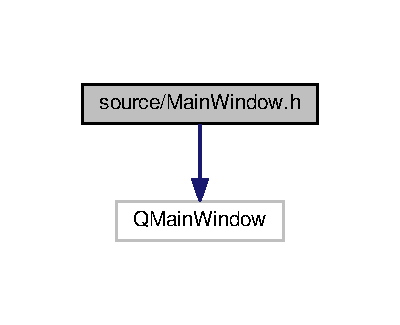
\includegraphics[width=192pt]{_main_window_8h__incl}
\end{center}
\end{figure}
This graph shows which files directly or indirectly include this file\-:
\nopagebreak
\begin{figure}[H]
\begin{center}
\leavevmode
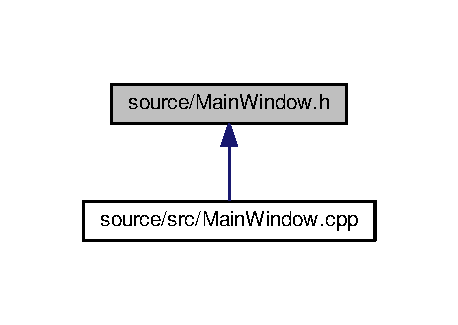
\includegraphics[width=220pt]{_main_window_8h__dep__incl}
\end{center}
\end{figure}
\subsection*{Classes}
\begin{DoxyCompactItemize}
\item 
class \hyperlink{class_main_window}{Main\-Window}
\begin{DoxyCompactList}\small\item\em The \hyperlink{class_main_window}{Main\-Window} class shows an example implementation of the Q\-S\-Ticky\-Button with all the capabilities used. \end{DoxyCompactList}\end{DoxyCompactItemize}


\subsection{Detailed Description}
Example implementation of the \hyperlink{class_q_sticky_button}{Q\-Sticky\-Button}. 

Definition in file \hyperlink{_main_window_8h_source}{Main\-Window.\-h}.


\hypertarget{_q_sticky_button_8h}{\section{source/\-Q\-Sticky\-Button.h File Reference}
\label{_q_sticky_button_8h}\index{source/\-Q\-Sticky\-Button.\-h@{source/\-Q\-Sticky\-Button.\-h}}
}


Sticky button that has click and hold capability.  


{\ttfamily \#include $<$Q\-Widget$>$}\\*
Include dependency graph for Q\-Sticky\-Button.\-h\-:
\nopagebreak
\begin{figure}[H]
\begin{center}
\leavevmode
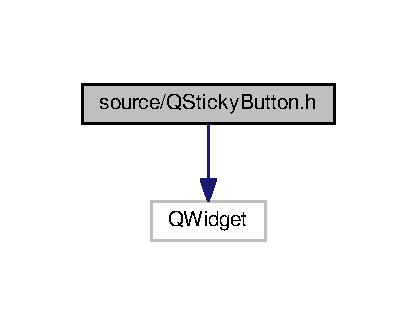
\includegraphics[width=200pt]{_q_sticky_button_8h__incl}
\end{center}
\end{figure}
This graph shows which files directly or indirectly include this file\-:
\nopagebreak
\begin{figure}[H]
\begin{center}
\leavevmode
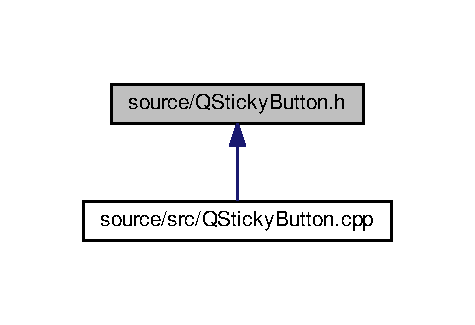
\includegraphics[width=228pt]{_q_sticky_button_8h__dep__incl}
\end{center}
\end{figure}
\subsection*{Classes}
\begin{DoxyCompactItemize}
\item 
class \hyperlink{class_q_sticky_button}{Q\-Sticky\-Button}
\begin{DoxyCompactList}\small\item\em The \hyperlink{class_q_sticky_button}{Q\-Sticky\-Button} class implements a custom button with click and hold capability. \end{DoxyCompactList}\end{DoxyCompactItemize}


\subsection{Detailed Description}
Sticky button that has click and hold capability. 

Definition in file \hyperlink{_q_sticky_button_8h_source}{Q\-Sticky\-Button.\-h}.


\hypertarget{_main_window_8cpp}{\section{source/src/\-Main\-Window.cpp File Reference}
\label{_main_window_8cpp}\index{source/src/\-Main\-Window.\-cpp@{source/src/\-Main\-Window.\-cpp}}
}


Example implementation of the \hyperlink{class_q_sticky_button}{Q\-Sticky\-Button}.  


{\ttfamily \#include \char`\"{}Main\-Window.\-h\char`\"{}}\\*
{\ttfamily \#include \char`\"{}ui\-\_\-\-Main\-Window.\-h\char`\"{}}\\*
Include dependency graph for Main\-Window.\-cpp\-:
\nopagebreak
\begin{figure}[H]
\begin{center}
\leavevmode
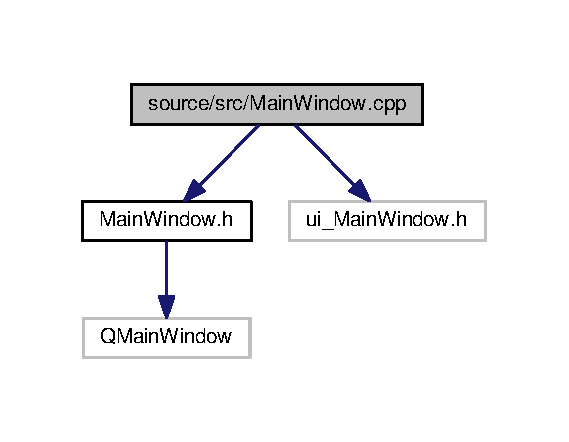
\includegraphics[width=273pt]{_main_window_8cpp__incl}
\end{center}
\end{figure}


\subsection{Detailed Description}
Example implementation of the \hyperlink{class_q_sticky_button}{Q\-Sticky\-Button}. 

Definition in file \hyperlink{_main_window_8cpp_source}{Main\-Window.\-cpp}.


\hypertarget{_q_sticky_button_8cpp}{\section{source/src/\-Q\-Sticky\-Button.cpp File Reference}
\label{_q_sticky_button_8cpp}\index{source/src/\-Q\-Sticky\-Button.\-cpp@{source/src/\-Q\-Sticky\-Button.\-cpp}}
}


Sticky button that has click and hold capability.  


{\ttfamily \#include \char`\"{}Q\-Sticky\-Button.\-h\char`\"{}}\\*
{\ttfamily \#include \char`\"{}ui\-\_\-\-Q\-Sticky\-Button.\-h\char`\"{}}\\*
Include dependency graph for Q\-Sticky\-Button.\-cpp\-:
\nopagebreak
\begin{figure}[H]
\begin{center}
\leavevmode
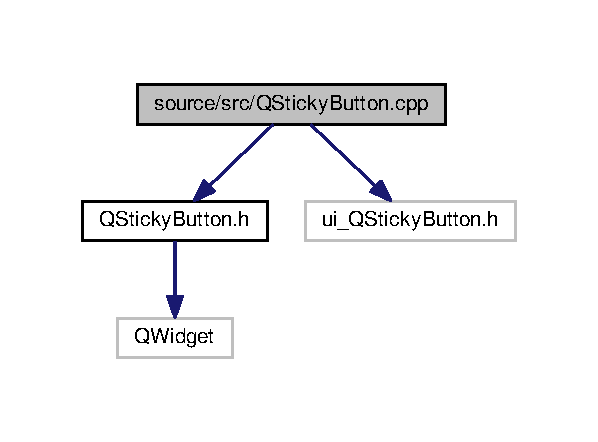
\includegraphics[width=287pt]{_q_sticky_button_8cpp__incl}
\end{center}
\end{figure}


\subsection{Detailed Description}
Sticky button that has click and hold capability. 

Definition in file \hyperlink{_q_sticky_button_8cpp_source}{Q\-Sticky\-Button.\-cpp}.


%--- End generated contents ---

% Index
\newpage
\phantomsection
\addcontentsline{toc}{chapter}{Index}
\printindex

\end{document}
